\documentclass[letterpaper, 10 pt, conference]{IEEEtran}

%% Language and font encodings
\usepackage[english]{babel}
\usepackage[utf8x]{inputenc}
\usepackage[T1]{fontenc}
%% Sets page size and margins
%% Useful packages
\usepackage{amsmath}
\usepackage{graphicx}
\usepackage{cite}
\usepackage[colorinlistoftodos]{todonotes}
\usepackage[colorlinks=true, allcolors=blue]{hyperref}
\usepackage{url}
\usepackage{hyperref}
\usepackage{float}
\usepackage{lettrine}

\title{Programming Languages Over the Years}
\author{\textbf{Nathan Donaldson}\\
Computer Engineering, University of Utah}

\begin{document}
\maketitle 	
\makeatletter
\def\ps@headings{%
\def\@oddhead{\mbox{}\scriptsize\rightmark \hfil \thepage}%
\def\@evenhead{\scriptsize\thepage \hfil \leftmark\mbox{}}%
\def\@oddfoot{\scriptsize \@date\hfil PLOTY}%
\def\@evenfoot{\scriptsize PLOTY...\hfil \@date}}
\makeatother

\pagestyle{headings}

\begin{abstract}
This survey goes over the history of programming languages. It goes over the many different languages that have come to fruition over the years: What they are, when they started, and a few features that they brought with them. It then proceeds to discuss what languages may be best for certain situations such as Web Development, Gaming, Hardware, Research, etc. Where will it go from there? What are the current trends? We discuss these few things last, because it's important to look at trends and where things might go if someone is interested in the field of software development. 
\end{abstract}

\section{Introduction}
\lettrine[findent=2pt]{\textbf{T}}{}here are many programming languages to pick from these days. They all stemmed and evolved from somewhere, and they are all starting to share the same human friendly approach to developers. Where did all these languages come from? When did it start? How have languages evolved? Where will they go? Many languages were developed by accident, some on purpose, maybe not knowing how widely used they would be. Programming languages were around since the very first computer was ever invented. Technically binary could be considered a programming language. We would probably not consider that the case today, but in the end thats what everything boils down to. Older languages are even still used today, evolving, improving due to communities and researchers. Its hard to tell what language might be the next popular one. 

\section{Language Time Line and Evolution}
\noindent \underline{Assembly} \\
Assemblers have existed from a very very early stage of computers, you could probably say the beginning. The Assembly language was pretty much the first language that associated a symbolic name to machine language code. It is so low level that it isn't practiced anymore. But you can learn alot from Assembly code, some schools give a taste of assembly to students so they may appreciate computer languages a bit more. A program written in assembly consists of a series of pseudo-instructions, comments, and data. Instructions usually consist of an operation code followed by a list of data, arguments paramaters. The command B0 61 tell an x86/IA-32 processor to move an immediate 8 bit value into some register.~\cite{History} So here the opcode is B0, which says move the hex value 61 into register AL.\bigskip

\noindent \underline{FORTRAN (Formula Translation)} \\
One of the oldest languages still in use,  created by John Backus in 1957, and developed to perform high level scientific, mathematical, and statistical calculations. FORTRAN is still used today in aerospace, auto industry, government and research institutions. Fortran intruduced sub-routines, functions, loops and a primitive FOR control structure. FORTRAN was designed to be an easy to learn, machine dependent, problem oriented language that permitted complex math functions to be expressed in regular algebraic notation.\bigskip

\noindent \underline{COBOL (Common Business Oriented Language)}\\
It's what is running behind a majority of business transaction systems, credit card processing, atm's, telephone/cell calls, hospital systems, government, automotive, traffic, etc. It was created by a team lead by Dr. Grace Murray Hopper in 1959 and it introduced the RECORD data structure. COBOL has an English-like syntax, which is used for everything in a a COBOL program. For example, instead of symbols, words were used to express conditional statements. Things like x > y could also be written as x IS GREATER THAN y. Many other words like IN, OF, ARE, VALUE, etc. were used.\bigskip

\noindent \underline{BASIC (Beginners All Purpose Symbolic Instruction Code)}\\
This language arrived in 1964. It was developed by students at Dartmouth College and was designed for people without a strong technical or mathematical background. Bill Gates modified this with Paul Allen and Microsoft's first product was born. It ended up being sold to M.I.T.S. for the Altair. Microsoft today still uses BASIC. Some significant features that BASIC had were loops, input from keyboards, menu driven applications, and system commands that would make the system perform specific tasks immediately. User defined functions, arrays, and sorting were also a big thing with the language. The language was aimed at students, since it became started to become popular on home computers. It was supposed to be easy to use, homework friendly, especially for non-science students. \bigskip 

\noindent \underline{C}\\
Declarations such as int or char were not created until around 1969 when C was developed. It was created by Dennis Ritchie at the Bell Telephone Laboratories to use Unix. It ended up becoming so great that the Unix kernel was rewritten in C. It was one of the first operating system kernels implemented in a language other than assembly. Linux today is still based on C. It is a great language with a lot of built-in functions and operators that can be used to write any complex program. It offers the capabilities of an assembly language with some higher level language features as well. Because of its closeness to assembly, it is the most used language in OS and embedded system development today.\bigskip 

\noindent \underline{Pascal}\\
Blaise Pascal was famous for inventing the first adding machine in 1641, and that is where the name PASCAL came from. Niklaus Wirth created Pascal as a teaching tool and it grew into widespread commercial use. Its goal was to make building compilers easier. It was a strongly typed language with extensive error checking. It offered several data types like arrays, records, files, sets, etc. It grew popular in academics because it was easy to learn, very structured, and could be be compiled on many platforms.\bigskip

\noindent \underline{C++}\\
This language came in around 1983, and was (still is) extremely popular along with C. Bjarne Stroustrup modified C to C++ and today it is still considered the most popular programming language ever created. It's used by things like Microsoft Office, Adobe PDF Reader, Firefox, etc. C++ brought about Object Oriented Programming to C and introduced operator overloading. It also brought about the use of Inheritance and templates, as well as encapsulation. Inheritance provides the idea of reusability and add new features to an existing class without modifying it. Encapsulation hid data from data structures and wrapped up data into a single entity, allowing only functions to access it.\bigskip

\noindent \underline{PERL}\\
Standing for Practical Extraction and Report Language, Perl came about when Larry Wall, a Unix programmer, couldn't extract data the way he needed and found that UNIX could not do what he needed. That's why the acronym is Practical Extraction Report Language. This language is used by the popular site Craigslist. It brought about the use of lists, associative arrays, and the foreach control structure. Perls database integration DBI supports many third-party databases such as Oracle, Sybase, MySQL, and many others. Perl works with well with HTML, XML, and other mark up languages as well. \bigskip

\noindent \underline{Python}\\
After a few years, PYTHON came around and basically replaced Perl. It's name was inspired by the Monty Python movie. It was developed by Guido Van Rossum to fix problems in the ABC language. He still serves as its lead designer today. Python is a simple language. Reading and coding is very much like english. It's simplicity allows you to focus on coding and not worry about the syntax itself. \bigskip

\noindent \underline{Ruby}\\
Languages started spreading from each other at this time by taking bits and pieces of other languages and implementing and improving upon them. Ruby was such a language that was developed by Yukihiro "matz" Matsumoto. He named the language after the birthstone of July. He ended up blending Per, Smalltalk, Eiffel, Ada, and Lisp together to create this. Those were his favorite languages.~\cite{History} Ruby reduced code size from python, statements were terminated by the end of a line instead of another symbolic terminator. Blocks of statements were ended with the "end" statement. Dynamic objects came from Ruby. Ruby is an open-source, general purpose, object oriented programming language similar to Python and PERL. Ruby is mostly used for developing web applications and has many built in functions that help make this easy for a programmer.\bigskip

\noindent \underline{PHP}\\
Rasmus Lerdorf created one of the most popular languages used in web architecture. PHP came around because he wanted to replace Perl scripts used to maintain his personal home page. Facebook is one big user of PHP. PHP brought about a multi-platform scripting language, embedded inside HTML. The interpreter parses an html page that embeds PHP and delivers a pure html page. It allowed webmasters to build dynamic pages. PHP is cross compatible, it supports usage of variables without declaring a data type~\cite{History}. It also has variable variables, which allows the changing of a variable name dynamically. REGEX methods are also integrated into PHP that have extensive parsing and speed. \bigskip

\noindent \underline{Java}\\
Now onto my favorite language, JAVA! A team at Sun Microsystems lead by James Gosling created Java to run set top boxes for interactive television around 1995. Java is vastly used and most websites cant function without it. It was even used on the Mars Rovers! One reason Java is so popular is because it an be interpreted on any computer. It has great auto memory management, and has no manual pointer usage. When it first came out it did not allow operator overloading, but it has evolved along with all languages. It offered dynamic arrays and integrated multi-tasking as well. It was designed with a small number of language constructs so programmers could have an easier time learning it. It eliminated things like goto statements, header files, pointers, and other things that required more maintenance\bigskip

\noindent \underline{Javascript}\\
Around the same time Javascript came! Javascript has nothing to do with Java and was used mostly for web development on the client side. It is a scripting language to embed procedural code into web pages. Later it found itself on the server side as well. It was originally developed by Brendan Eich of Netscape under the name Mocha. Javascript syntax is highly influenced by C's syntax.~\cite{History} It may be used in other XML based based language applications as well. It has untyped variables, and instead web pages are accessed through the document object model. Javascript is popular because of its browser support, client/server side uses, support for objects, and its overall functionality as a programming language. \bigskip

\noindent \underline{C\#}\\
In the year 2000 C\# was developed. It became the main language of the .NET environment, to program software working through the web. C\# has a C and Java syntax, but like Java, has a garbage collector, no pointers, multitasking, and interfaces. Structs were a special object, passed by values. Literals were objects as well with methods. Attributes and properties were also introduced in this language. Delegates are a powerful tool as well in C\# and replaced pointers of functions in C. C\# is a simple, modern, object oriented, type safe language. \bigskip

\noindent \underline{Ruby on Rails}\\
Now back to Ruby... Ruby is most famous for its framework Ruby on Rails. It was developed by David Heinemeier Hansson from his work on Basecamp in 2005, a project management tool by 37signals. Ruby on Rails makes web devopment much easier, especially for people who are not experts in the web development world. Some of Ruby on Rails main features are its MVC architecture, Database Access Libraries that simplify data handling in databases, its convention or configuration rule, which excludes XML and uses simple programming conventions to specify configuration parameters.\bigskip

\noindent \underline{GO}\\
Developed by google around 2009, it is a modified language from C++ but without header files and simpler syntax. There really wasn't anything new with GO, it was designed specifically for compilation speed. Go generates binaries that include everything so you don't have to install runtime's that are needed for your application. Parallelism is emphasized in the language. Any function may be executed as a "goroutine" by prefixing a function with "go". The language also has a "channel" feature that can pass data in and out of the goroutines. The specification when it comes to design is short and sweet, and their mantra is to "do more with less".\bigskip

\noindent \underline{Swift}\\
If you are an iOS software developer, than you are probably familiar with the new language SWIFT. It was developed a few years ago and basically replaced Objective-C on apple devices. Objective-C is still the core of iOS so it wont be going away anytime soon most likely. It has a classic design and changed the name of elements, setting itself apart from other languages. One example is renaming interfaces to protocols. Swift is fast, safe, and expressive, with features such as multiple return values, tuples, functional programming patters, and powerful error handling.~\cite{History}
\bigskip

\indent The invention of languages have not changed the application of instructions, just the difference in more human readable code and less management is more common as time goes on. There are 3 big types of languages over the years that were developed. Object Oriented, Scripting, and Markup. Object Oriented languages allow embedding code inside HTML pages, as well as use in many other applications. PHP, ASP, and Javascript are the most common. Classes are being replaced by dynamic objects and inheritance by combination. Scripting languages, in the 2000's, offered a simpler syntax. Python is the most widely used for now but is slowly being replaced by Go. Markup Languages were a huge trend from 2000 to 2010 but it was dedicated to graphical interfaces. JSON has been the replacement of this. SQL trends are becoming popular now as well and are becoming a part of everyday modern programming.
\indent Overall, over the span of computing languages have evolved from creation of high-level languages, expansion of specialized languages, duels between languages, experimenting with objects, generalization of object oriented programming, web development, and concurrency. 


\section{What to Use}
\indent I'm going to end this paper with a few topics, one of which is what languages are best for which situations. Now, its not easy to say which language is the "best" because it really depends on how you harness each language and how well you maintain and build upon what you are using. There are many different choices of languages to choose from, and some languages are better in certain criteria compared to others. You wouldn't want to use a language that was created for web development for game development, but it can be used in that fashion, it just wont behave as well or most likely wont do what you want it to do. You could always develop a new language i suppose. In a company environment, changing languages costs money, and in the same way, money can change languages. Things such as technical qualitites, platform support, the work your doing, your customer base size, etc. come into play. The popularity of a language can also help. Taking advantage of open source development, libraries that have already been written and are open for use, and large communities that help each other with problems are a big perk of popular languages. 
\newline
\subsection{For Enterprise and Research}
\indent If you are in an environment that uses a lot of hardware, C and C++ are really good languages to use mostly because they are lower level languages and have a lot more power. C and C++ require a lot more knowledge and understanding than higher level languages though. These languages still continue to improve in both code and compilation. There are some disadvantages that will require you to force your way through, but maintenance is much more difficult as well. Python is a great language that is widely used in many different fields because it is easy to extend and embed. It is very popular because it is designed to be fun to use, as well as easy to read. It is mostly used in several areas of AI, from machine learning to language processing. The bad part of Python or any higher language is the performance compared to lower level languages. Python is not standard yet and there isn't an easy way to deploy Python applications. Version 3 is incompatible with previous versions and is still having problems. ~\cite{TheBest}But most languages always need work and improvement.  Julia is used for high-performance scientific computing and some simple web development. It has more performance and is less popular than Python. It also supports parallelism and the ability to call C, Fortran, and Python code directly.~\cite{TheBest} It is often used together with Python. Some other small languages like R and Matlab are used for complex mathematics. They are technically programming languages but are used more for research and development. If you are familiar with Java, Kotlin is a way to get partially out of it. Kotlin is designed to be safer and more productive than Java and is 100\% compatible with Java. It is now the second language to be supported by Android. It is fairly new as well. I have come to learn that Kotlin is quite powerful and reduces Java code by a lot.
\newline
\subsection{System Hardware Software}
\indent System software is software used primarily by other programs. It needs performance that is close to hardware. If you work with system software, you are the one hat has to deal with all the hardware differences so that everybody else can work productively. C was basically the language that eliminated all of its competitors at the time when it came to interfacing with hardware. It has a few issues, mostly manual memory management. If you are coding in C, you will most likely need to have a lot of experience because the language does not help you in any way. C++ is a step up from C and has an advantage of supporting larger applications because it supports object oriented programming, but it isn't re ally necessary. Rust is a new language sponsored by Mozilla for system programming. It is open-source and open to the community. It is loved by many users and is the "most loved programming language"~\cite{Stats} according to a survey of developers by StackOverflow. See Figure \ref{fig:Most Loved}
\begin{figure} [!ht]
\centering
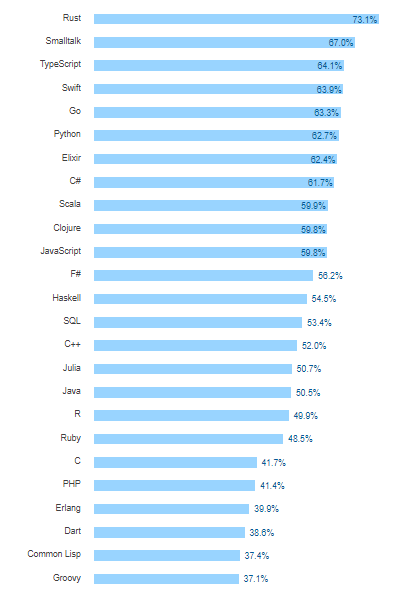
\includegraphics[width=0.4\textwidth]{mostLoved.png}
\caption{}
\label{fig:Most Loved}
\end{figure}
\newline
\subsection{Game and Web Development}
\indent Game development is based more around hardware than anything, but software does make development easier depending on what you are using. Simplifying game development by developing easy to use game engines makes a big difference. C++ is the most used programming language for professional game development. C\# is also used and is easier for developing across multiple platforms.  Javascript is basically the only choice for client-side web development, but is also used server-side. There are web frameworks for all kinds of applications, from complicated to simple ones. Javascript ended up spreading to the server side because of its optimization of runtime environments and development~\cite{TheBest}. C and C++ can claim a similar level of importance, but Javascript is used for the most part, especially by people with no previous experience or education in it. PHP was designed to simplify and speedup server-side web development. PHP wasnt every really designed to be a language and is considered badly designed. It works, no super efficiently, but it worked where nothing else would. Not until recently was it the only easy way of doing things server side in web development.
\newline
\subsection{Apple Software}
\indent Swift is a newer language and is the most loved language among Apple developers. Although Apple might decide to deprecate  Objective-C, it probably wouldn't happen, or at least anytime soon due to the fact that a lot of the codebase was written in Objective-C. You will get better performance, but the language is considered one of the most dreaded programming languages.
\newline
\indent You can use many languages in many applications, and it comes down to preference a lot of the time. Some might think other languages are better than others, but it really comes down to how well things are developed and structured. Languages are popping up and things can constantly change. The languages that have stuck around consistently the longest have been C and C++.\newline

\section{Where Will It Go}
\indent It's really hard to tell where programming languages are going to go and what will become popular or not. When social erupted, more web development languages like Javascript took off. But there are many factors that come into play: Generality, Reliability, Maintainability, Efficiency, Simplicity, Machine/Platform Dependencies, and Influence/Impact. These are just a few out of many reasons languages take the development path that they do. A language can achieve generality by taking many things and condensing them into one. If a language can reduce the amount of code needed to perform a specific task, it becomes more valuable.~\cite{ProgrammingLanguageTrends} The more reliable a language is to a specific industry increases value. Things like deprecation happen with many of today's languages, which can cause problems if it what takes its place does not perform the same. Maintaining things like memory was a large amount of work in older languages. Reducing the amount of work needed to develop is definitely important. Some languages are made to focus more on compiling time, runtime, memory allocation, etc. Which will you need more? Simplicity is a large one. The more time goes on, languages have been becoming more human readable that they were before. C and C++ are one of the most used out of older languages today, but that is due to the amount of power they have, and they have a decent language decent enough for humans to read. The wider range of products and platforms a language can run on is can make a huge difference. It really all just comes down to what's in demand. How many companies are using it? Whats easiest to use? What is in demand with consumers? I guess we will see where it goes. Figure \ref{fig:Language Over Time} a graph taken from stackOverflow about the change over the last 5 years in language popularity.~\cite{Stats} You can find a lot of interesting graphs on this site. 
\begin{figure} [!ht]
\centering
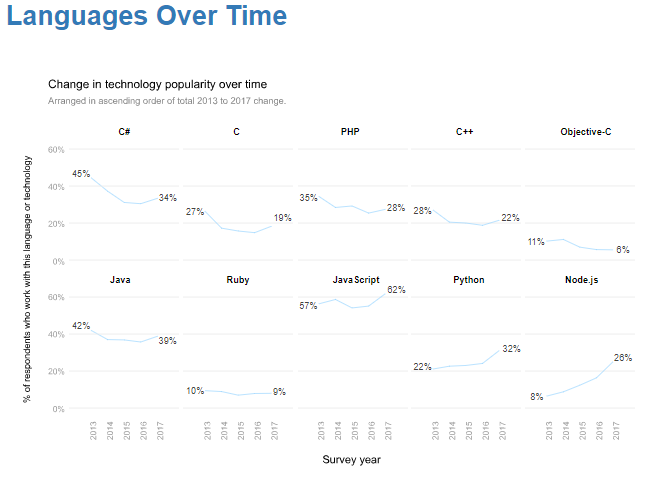
\includegraphics[scale = .9 , angle = 270]{languageOverTime.png}
\caption{}
\label{fig:Language Over Time}
\end{figure}
\newline


\section{What Is Popular today}
\indent What languages are popular to learn today? I would say Java is one of the most popular. Not only because i love it, but because its true. Its used for building server side applications, video games, mobile apps. It is the core foundation of Android apps and it runs across multiple platforms. Python has a lot to offer as well. There's a Python framework for almost anything. From web apps to data analysis. Python is said to be one of the easiest languages to learn and that is probably why it is most commonly taught in schools. It has risen more in popularity since Google started investing in it. C is very powerful if you work in hardware and is probably the most popular for that situation. It is difficult to master but is very powerful. Ruby is a leading supplier of web applications. It is easy to learn and has power, especially thanks to the Ruby on Rails framework. It is becoming more popular as time goes on. C\# is very closely related to Java but is meant for Microsoft, so if you enjoy Java, you can learn C\# pretty quickly. PHP is a must learn language for web developers. It is usually used with data heavy websites and app development. It has a ton of power. Objective-C and Swift are two that you would have to learn if you want to become an iOS developer. SQL is a database query language that associates with big data. It is used in just about anything that has a database backend, which is mostly anything.~\cite{TheBestToday}

\section{Conclusion}
It's crazy to see where languages have gone over the years, especially since they are all doing the same thing. If we stripped down every language that has been created, it all gets reduced down to 1's and 0's. But layer upon layer have been built upon one another to create these languages that compile and get reduced down to machine language behind the scenes. If you ever get to experience the inner workings of a computer, you will gain a much larger appreciation for what computers do for us. It truly is fascinating. From what i see, language development is all about making it easier for us as humans and that is it. I feel it will get to a point where everyone will be able to code anything they want easily and there wont be as high of a demand in developers. Web development is very popular due to the social media boom mobile applications. It will probably stay that way for awhile and i guess we will see where it goes. People who have experience in older languages will always be more valuable though, because older languages will always be being used since everything was built upon them. So far, my favorite languages have been Java, C\#, Kotlin,and Verilog. The only reason i would say they are my favorite is because i have enjoyed the time i have had developing with them. Getting more languages under my belt is always something i'm looking forward to.

\nocite{*}
\bibliographystyle{IEEEtran}
\bibliography{bib}

\end{document}